\chapter{Numerical Experiments}

\begin{table}[h]
    \centering
    \caption{Comparison of NDCG score across different model sizes and similarities}
    \begin{tabular}{lcccc}
    \toprule
    Model & NegEuclid & InvEuclid & Cosine & Dot \\
    \midrule
    Llama 3.2 1B & 0.921 & 0.912  & 0.952 & 1.000 \\
    Llama 3.2 3B & 0.934 & 0.926  & 0.969 & 1.000 \\
    Llama 3.1 8B & 0.120 & 0.113  & 0.093 & 0.091 \\
    \bottomrule
    \end{tabular}
    \label{tab:pretrained_last_hidden_scores}
\end{table}

% НЕ пытайся заменить \cite{TODO} на что-то осознанное, я это сделаю сам потом
The numerical experiments were conducted using Python and widely recognized deep learning libraries PyTorch\cite{torch} and Torch-Lightning\cite{torch-lightning}. For experiments with pre-trained models, Llama 3.2 1B, Llama 3.2 3B, and Llama 3.1 8B \cite{llama32} were utilized. For training models from scratch, a small LLama-like model with 150M parameters was employed (model config described in \ref{app:architecture_150m_llama}). The SlimPajama dataset \cite{slimpajama} served as the training data. Each model trained from scratch processed 1.5B tokens during training. After training, the models were evaluated on benchmarks including MMLU\cite{mmlu}, AGIEval\cite{agieval}, and SQuAD\cite{SQuAD}. The computational setup consisted of a single Nvidia 3090 GPU. The training and evaluation code is available on \href{https://github.com/PavelShtykov/research_tad}{GitHub}.

\section{Correlation Between Final Hidden States and Token Embeddings}

\begin{table}[h!]
    \centering
    \caption{Comparison of validation loss and score on benchmarks across 150M Llama-like model with different LmHead}
    \begin{tabular}{lcccc}
    \toprule
    LmHead Type & Loss $\downarrow$ & MMLU (5-shot, acc) & AGIEval (4-shot, acc) & SQuAD (1-shot, em) \\
    \midrule
    (base) LmHead           & 2.84 & 27.34  & 20.1 & 25.34 \\
    $\text{LmHead}_{tied}$  & 2.89 & 27.11  & 20.3 & 24.55 \\
    KnnHead                 & 3.01 & 26.80  & 19.9 & 25.08 \\
    \bottomrule
    \end{tabular}
    \label{tab:scratch_last_hidden_scores}
\end{table}


For pre-trained Llama family models, the NDCG score between model logits and various similarity metrics was measured. The detailed methodology is described in section \ref{final_hidden_method}. The metric was evaluated on a subsample of 1000 examples from the validation portion of the SlimPajama dataset. Averaging was performed across 100 tokens in the prompt and 20 generated tokens.


Based on the results in Table \ref{tab:pretrained_last_hidden_scores}, the following conclusions can be drawn:
\begin{enumerate}
    \item For Llama 3.2 1B and Llama 3.2 3B models, all similarity metrics rank tokens very similarly to how tokens are ranked by the standard model logits. This behavior is likely due to these models being trained by their authors with weight tying. The NDCG score of 1.0 for dot similarity confirms this.
    \item The Llama 3.1 8B model was trained without weight tying. For this model, the NDCG score for all similarity metrics proved to be extremely low. This indicates that the model itself does not attempt to bring final hidden states closer to the most probable tokens according to any proximity metric.
\end{enumerate}


\begin{figure}[t]
    \centering
    \begin{minipage}{0.48\textwidth}
        \centering
        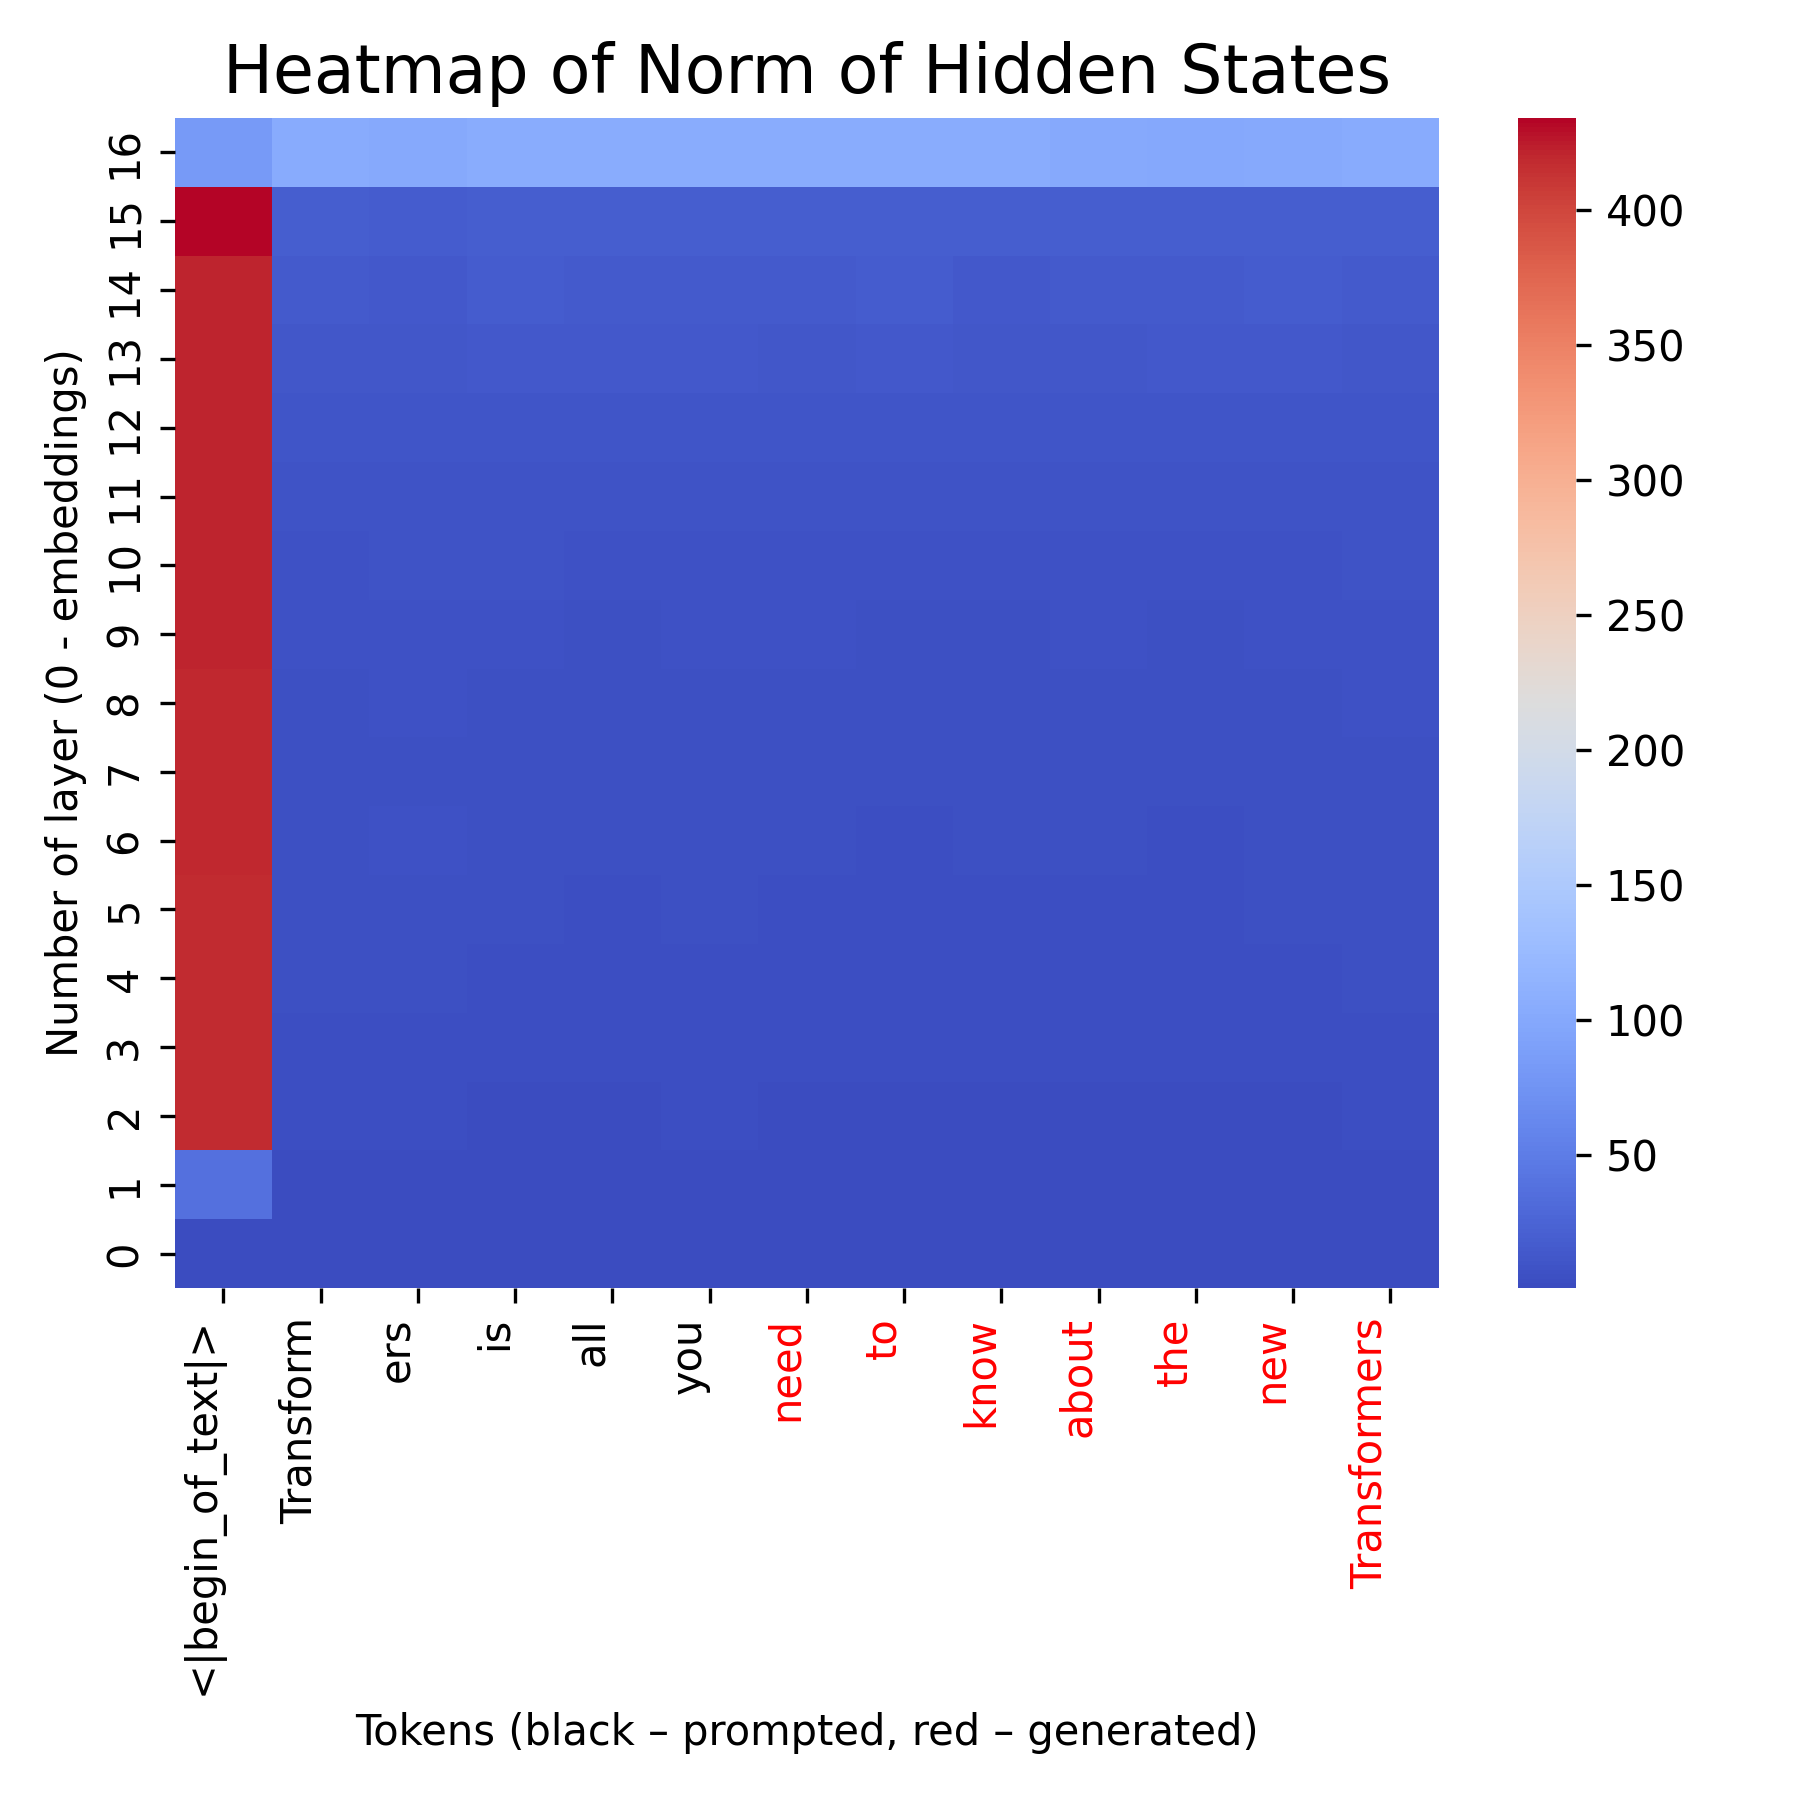
\includegraphics[width=\textwidth]{images/heatmap_1b_full.png}
        \caption{Heatmap of hidden state norms across layers and tokens for Llama 3.2 1B model. The x-axis represents tokens in the sequence (with generated tokens in red), and the y-axis represents model layers (with 0 being the embedding layer). Brighter colors indicate larger norms.}
        \label{fig:heatmap_1b_full}
    \end{minipage}
    \hfill
    \begin{minipage}{0.48\textwidth}
        \centering
        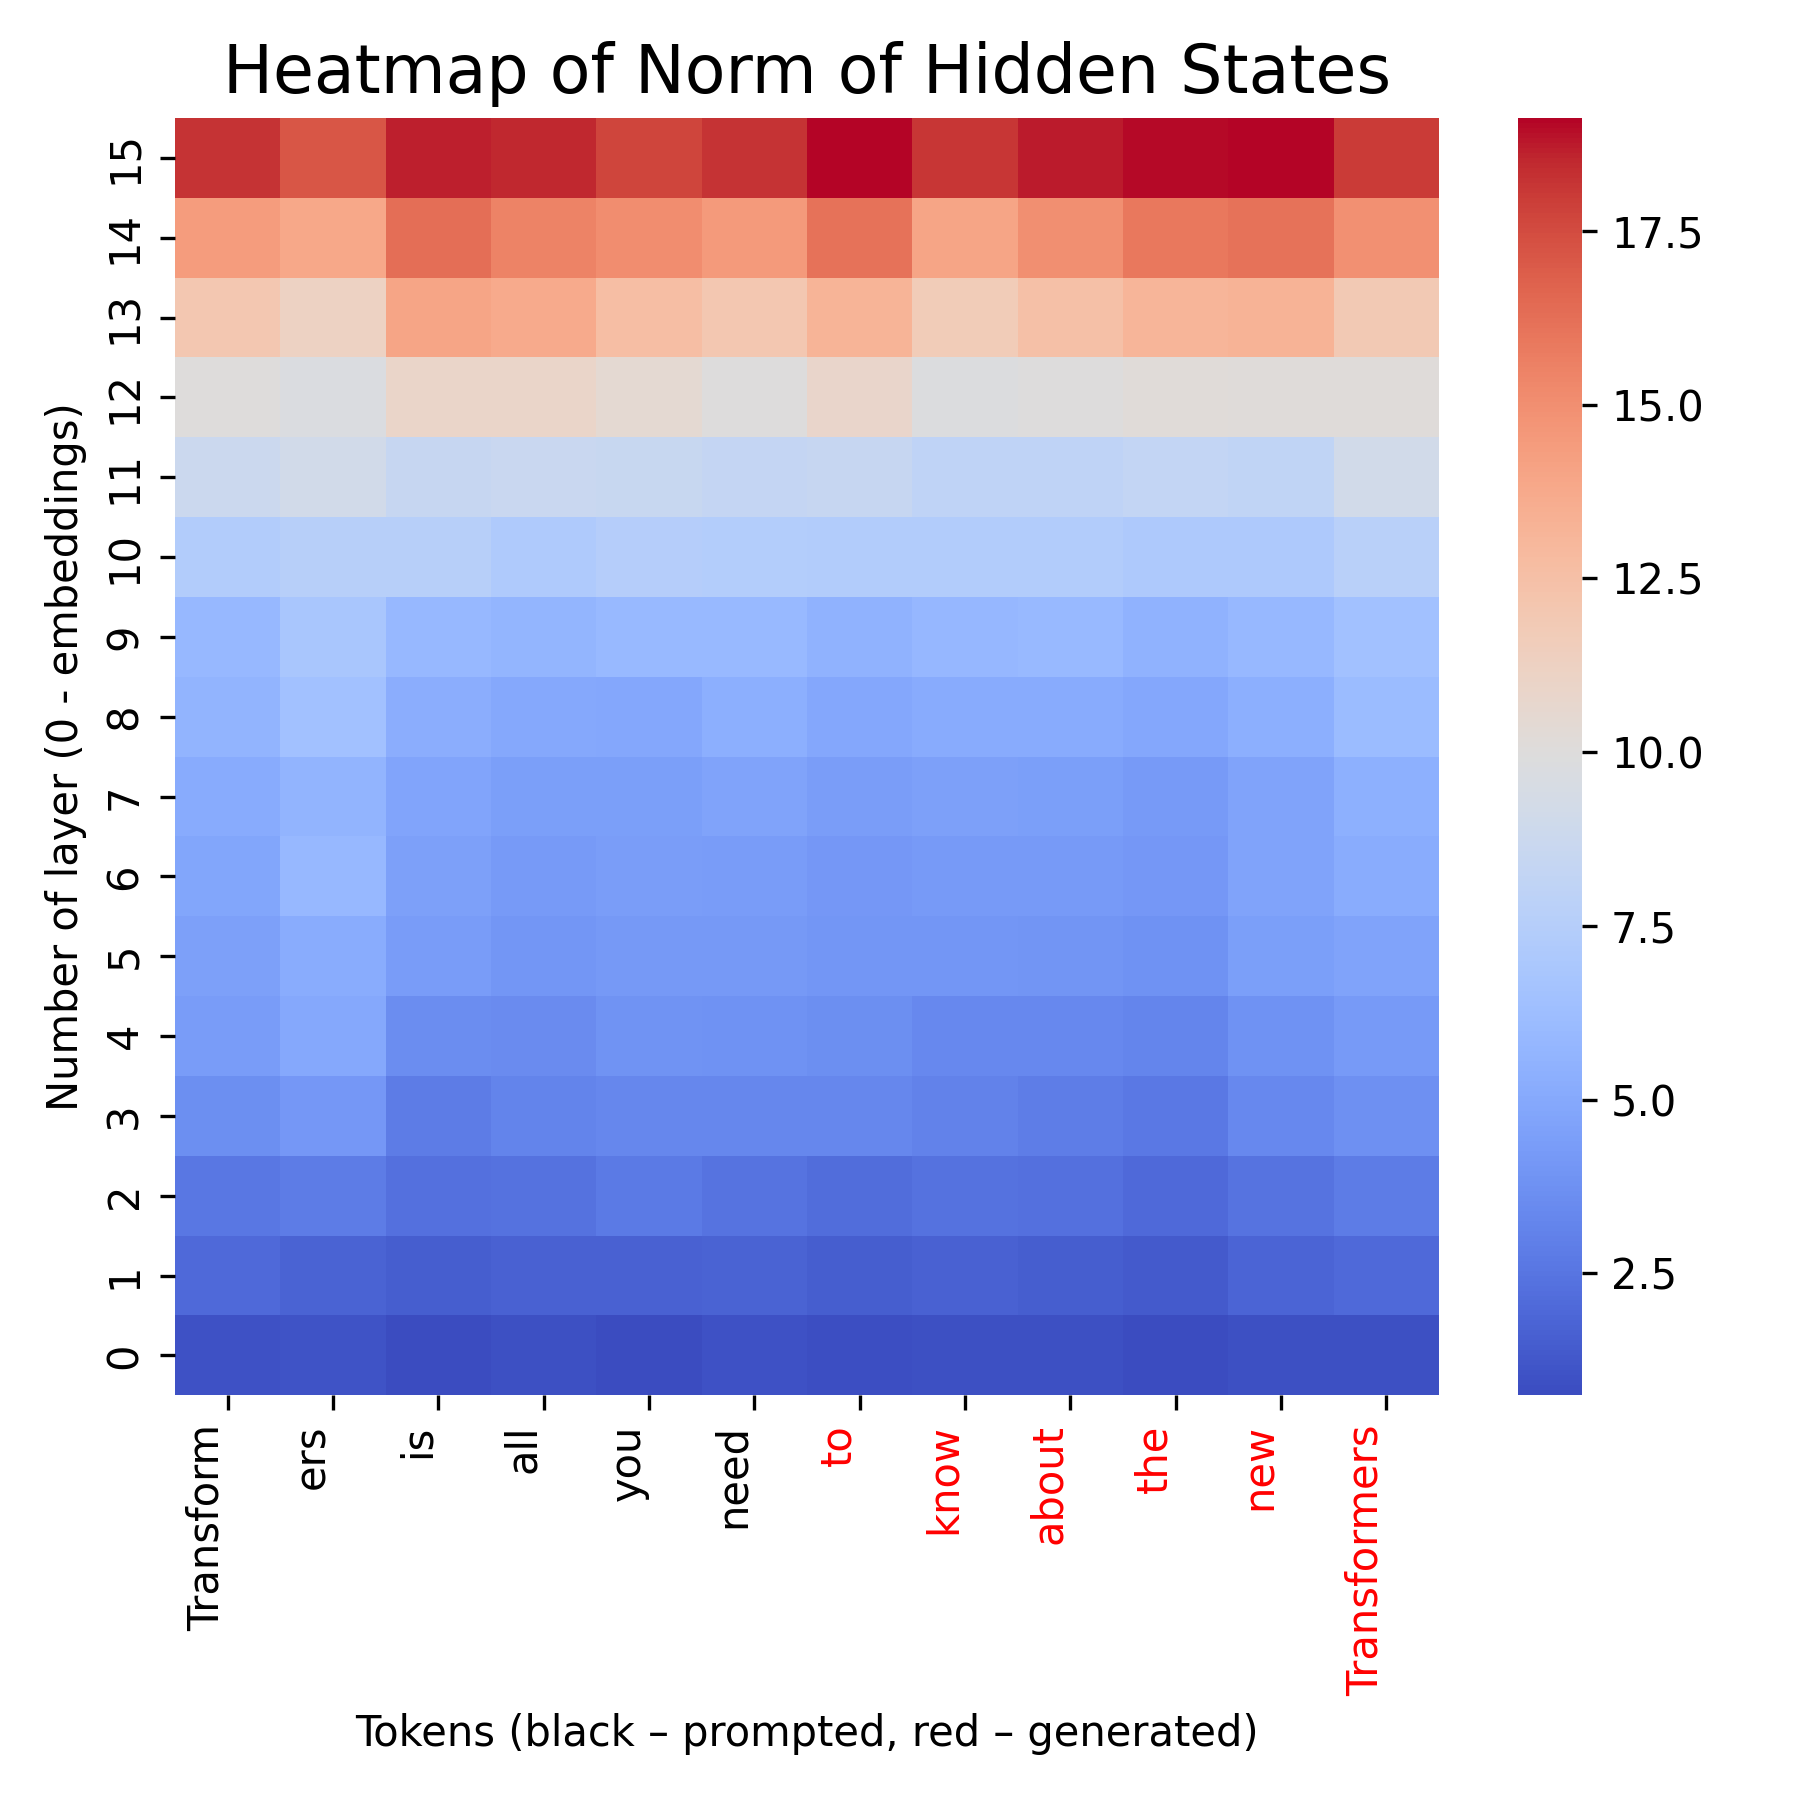
\includegraphics[width=\textwidth]{images/heatmap_1b_notfull.png}
        \caption{Heatmap of hidden state norms excluding the <BOS> token and final layer, providing a clearer view of the norm distribution in intermediate layers. Note the gradual increase in norm magnitude as layer depth increases.}
        \label{fig:heatmap_1b_notfull}
    \end{minipage}
\end{figure}


Several models were also trained from scratch with different variants of LmHead and their quality was measured on the validation set and standard benchmarks. A detailed description of the language head variations used in the experiments can be found in section \ref{scratch_final_hidden_info}.


The experimental results presented in Table \ref{tab:scratch_last_hidden_scores} reveal several significant findings:
\begin{enumerate}
    \item The standard LmHead configuration (without weight tying) demonstrated marginally superior performance across evaluation metrics. Nevertheless, all architectural variants maintained functional integrity and exhibited comparable performance characteristics, suggesting robustness in the underlying approach.
    \item All models converged to validation loss values consistent with expectations for models of this parameter scale (according to \cite{scaling_law}). This convergence pattern confirms the viability of all three architectural approaches for language modeling tasks.
    \item Performance on the AGIEval benchmark approached random baseline levels across all model variants. This observation indicates either inherent limitations in the model capacity relative to the benchmark complexity, or insufficient contextual information provided by the 4-shot prompting methodology.
\end{enumerate}

\section{Distribution of Intermediate Hidden States in Embedding Space}

\begin{figure}[t]
    \centering
    \begin{minipage}{0.48\textwidth}
        \centering
        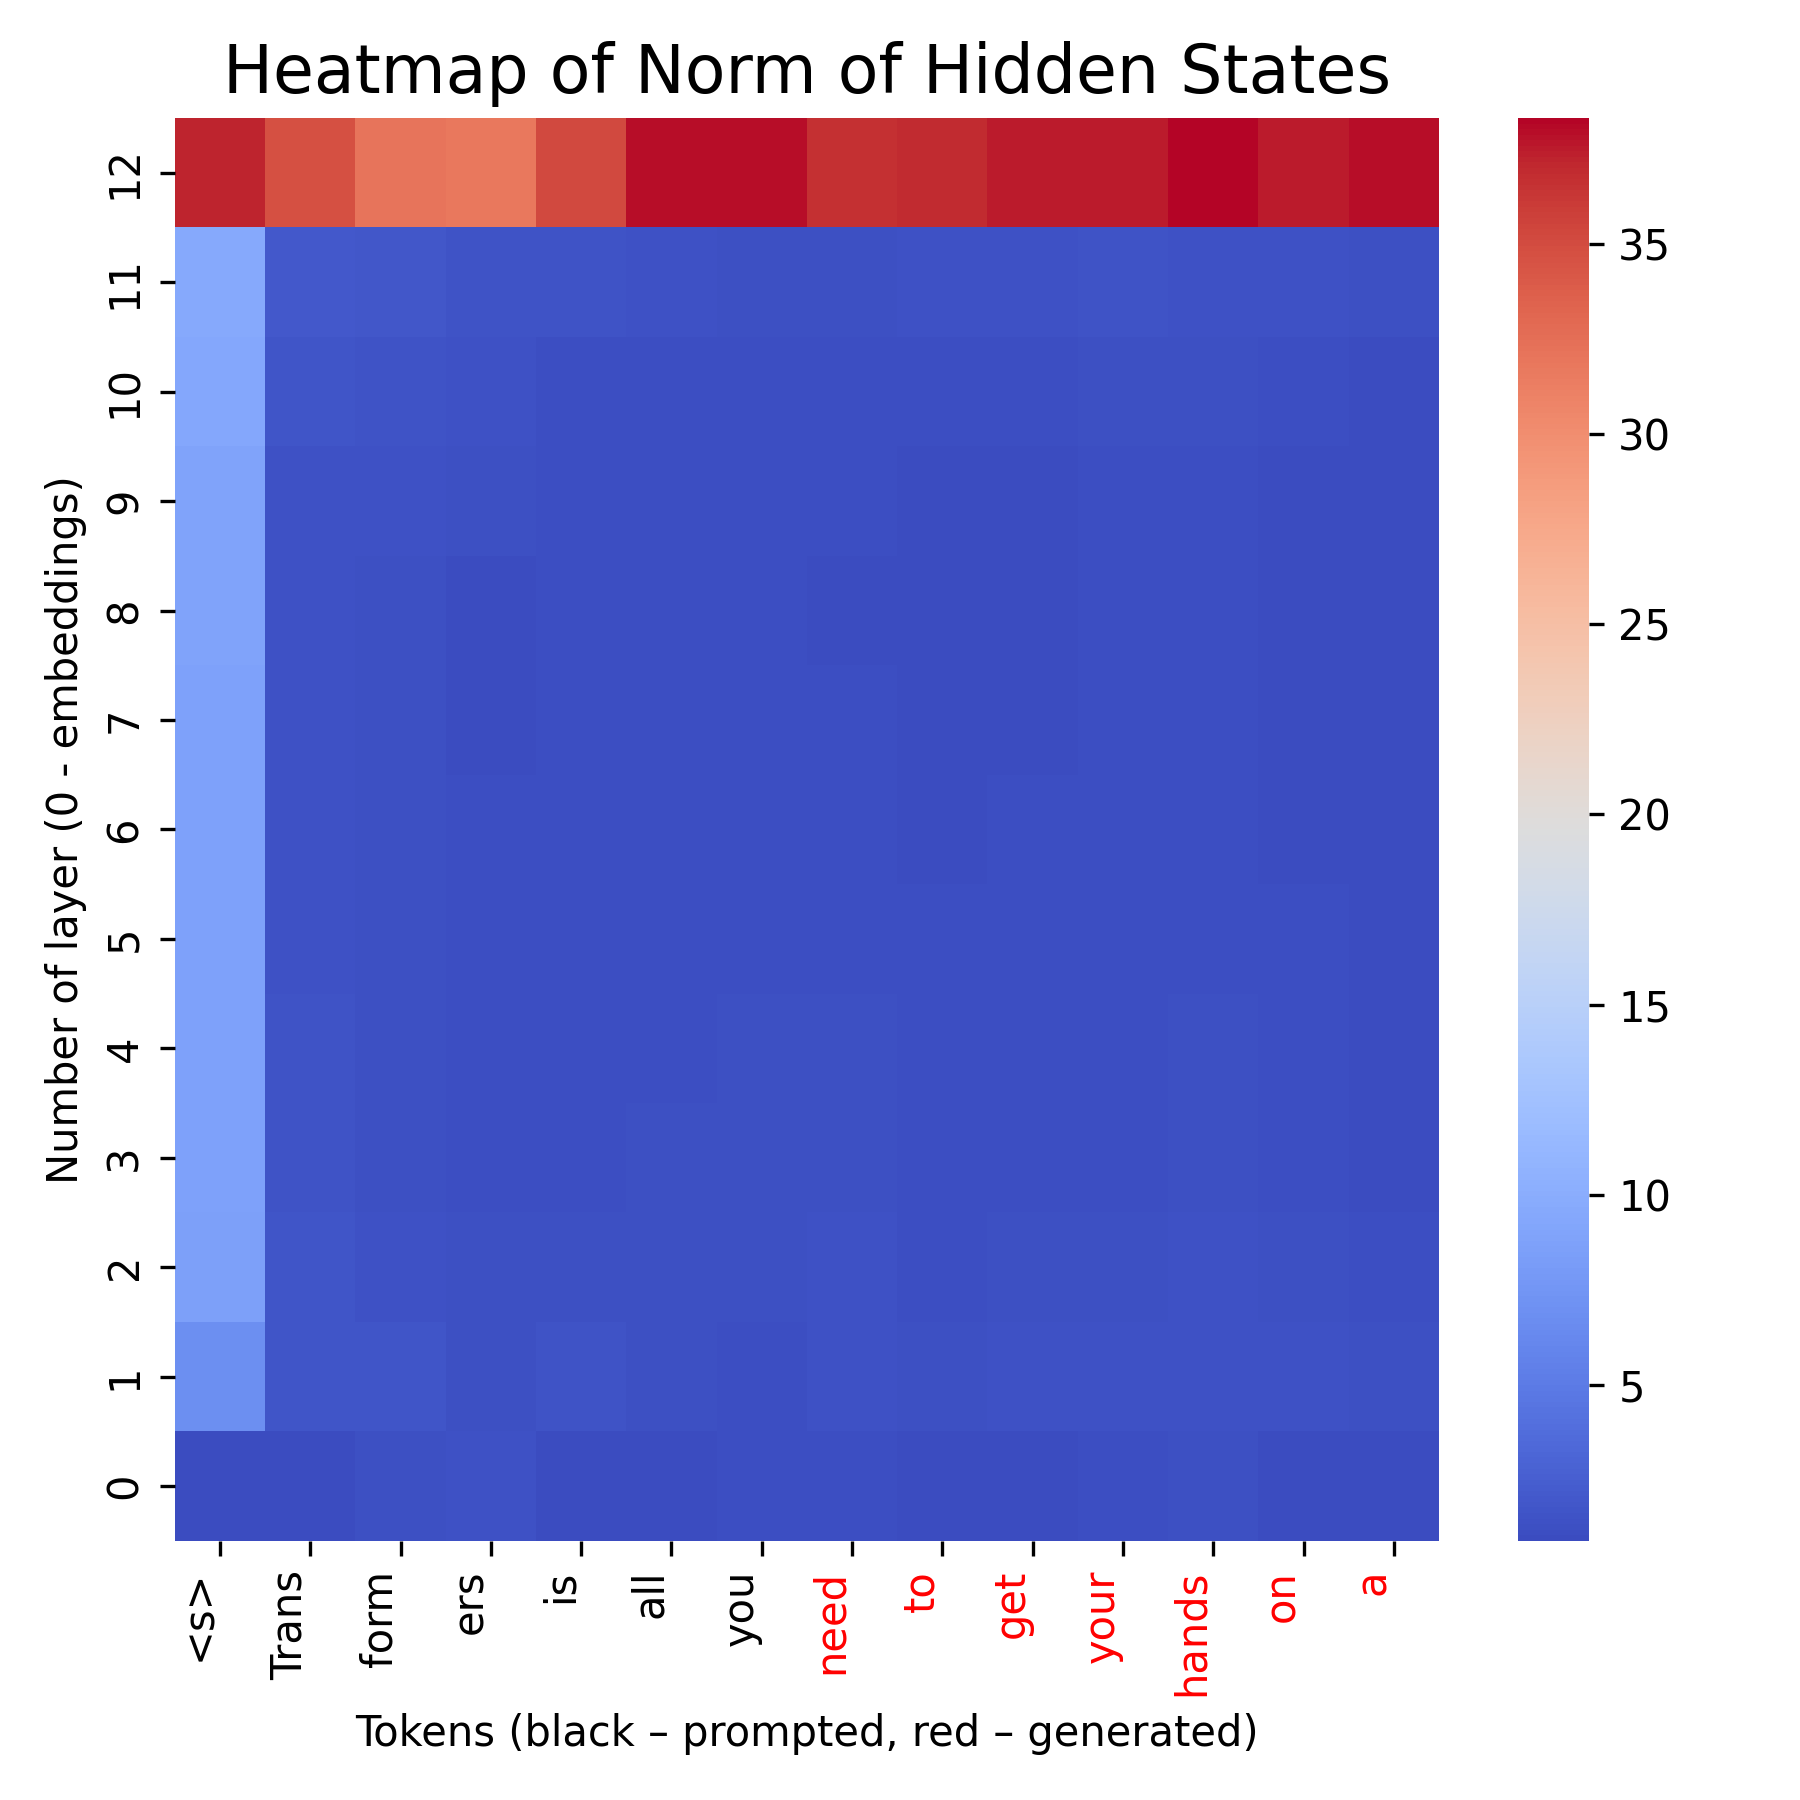
\includegraphics[width=\textwidth]{images/heatmap_150m_reg_all.png}
        \caption{Heatmap of hidden state norms for the 150M parameter model trained with the regularizer.}
        \label{fig:heatmap_150m_reg_all}
    \end{minipage}
    \hfill
    \begin{minipage}{0.48\textwidth}
        \centering
        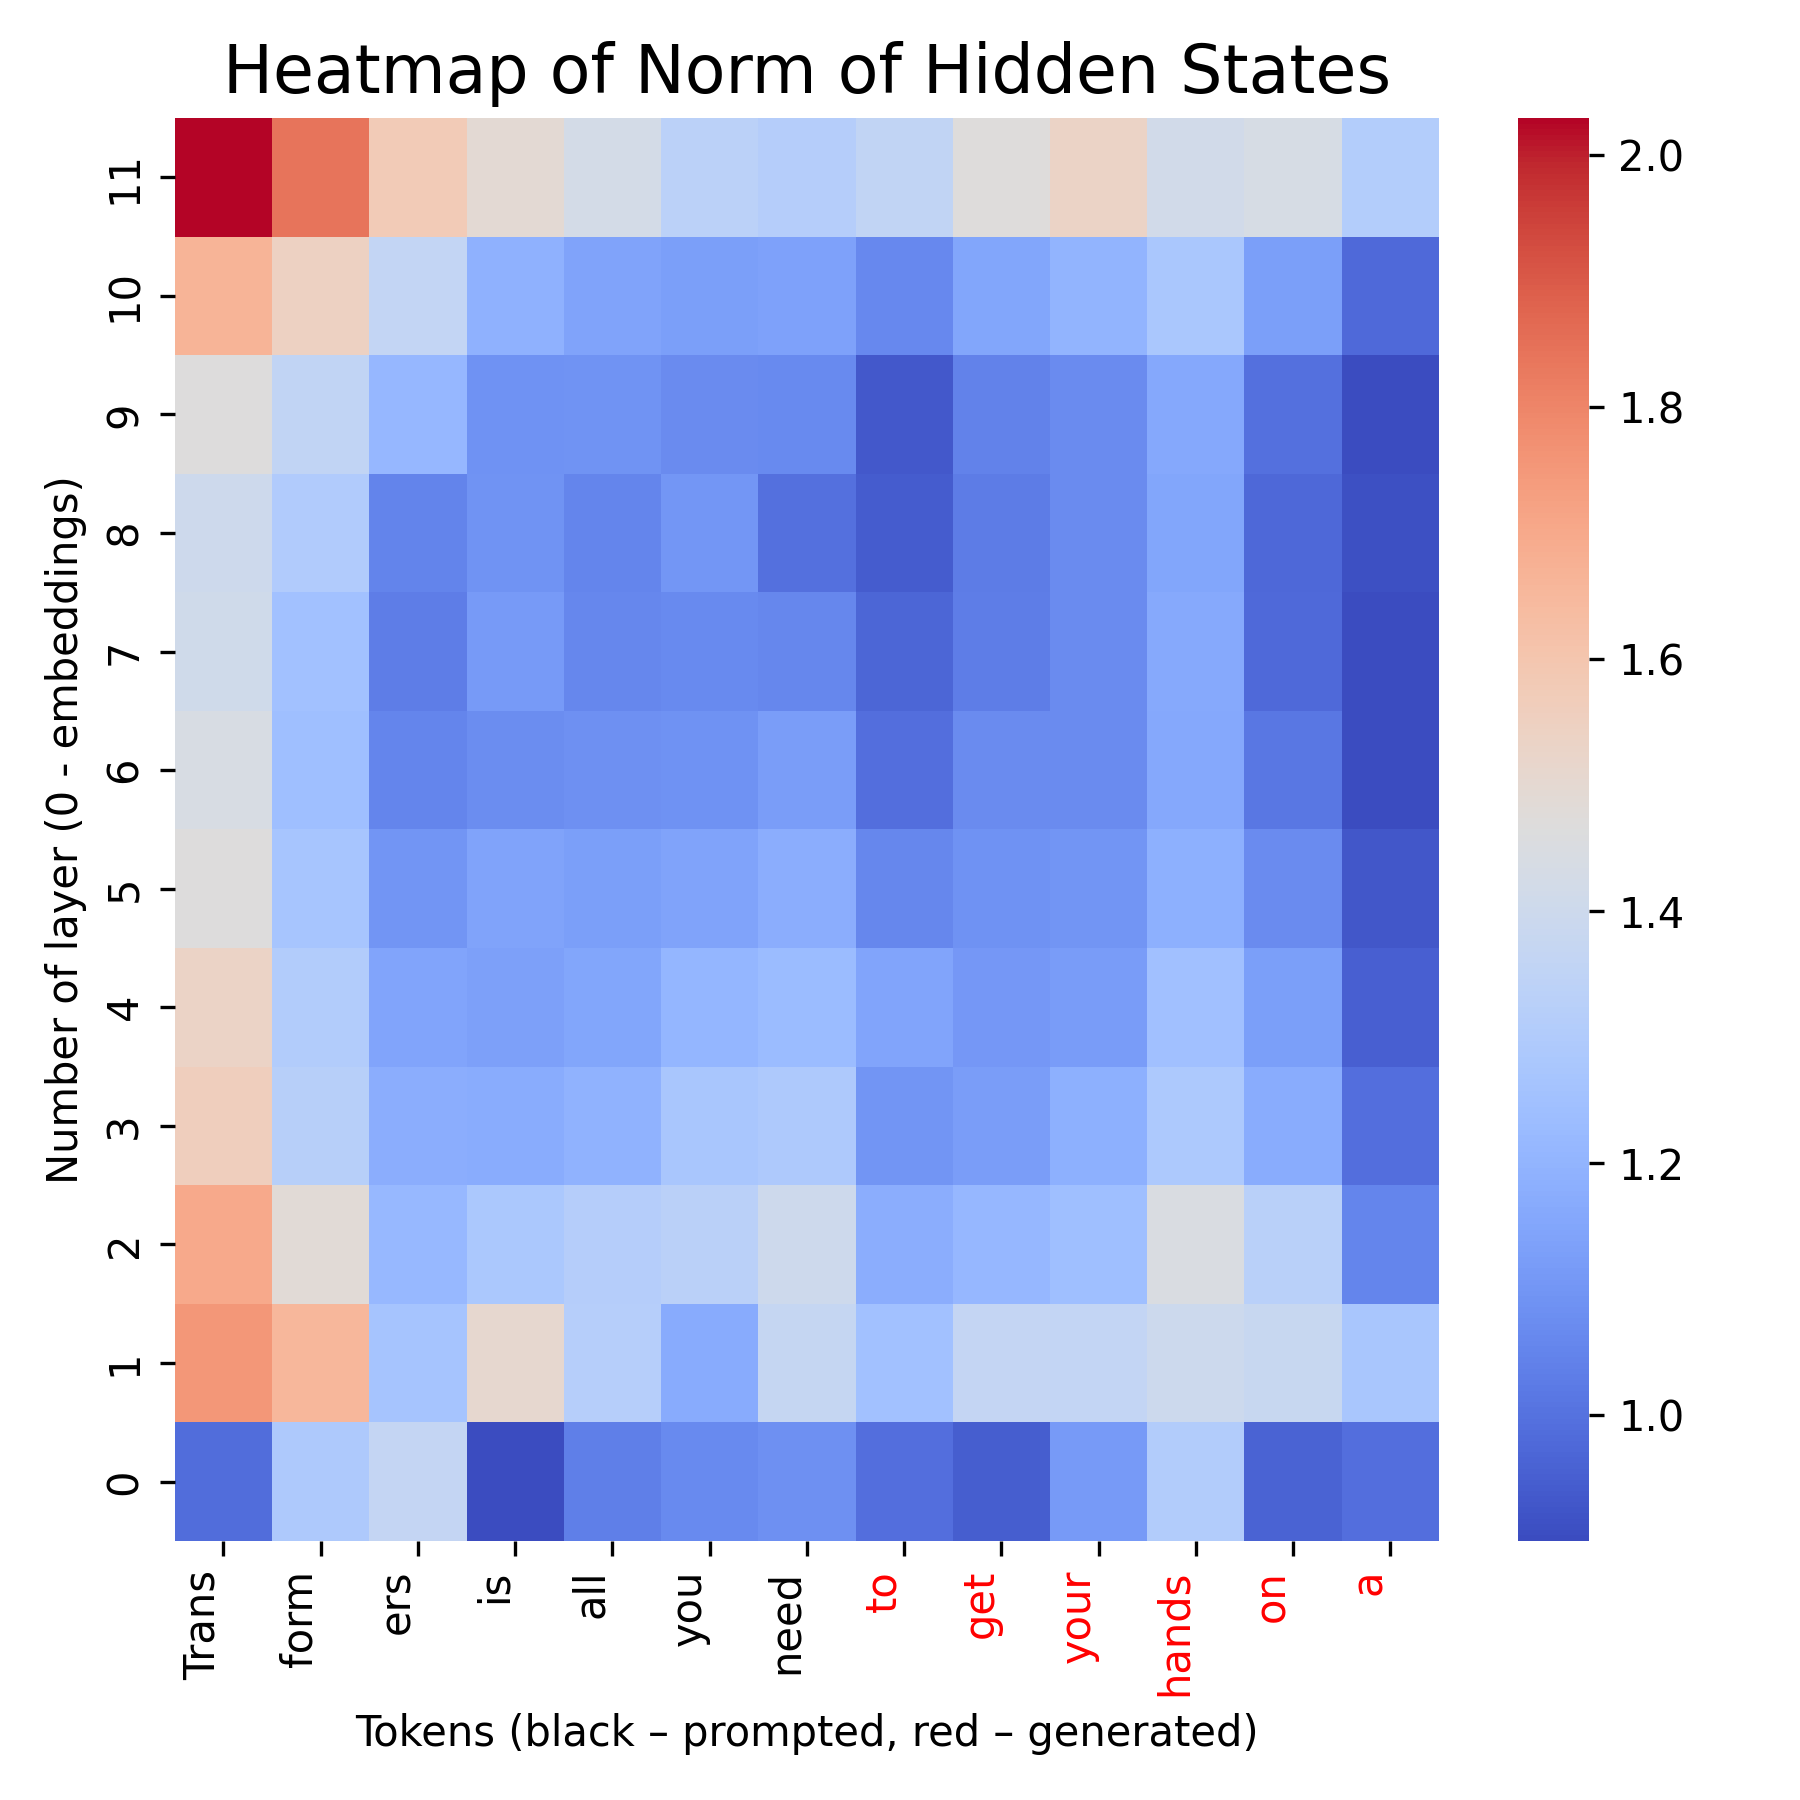
\includegraphics[width=\textwidth]{images/heatmap_150m_reg_notall.png}
        \caption{Heatmap of hidden state norms for the regularized model, excluding the <BOS> token and final layer. The regularization effect is visible in the more uniform norm distribution across layers compared to Figure \ref{fig:heatmap_1b_notfull}. All intermediate hidden states maintain norms comparable to token embedding norms (layer 0)}
        \label{fig:heatmap_150m_reg_notall}
    \end{minipage}
\end{figure}


To investigate the relative positioning of intermediate hidden states and token embeddings, the norms of hidden states after each layer of the model were visualized. For this visualization, the pre-trained Llama 3.2 1B model was initially used.

In Figures \ref{fig:heatmap_1b_full} and \ref{fig:heatmap_1b_notfull}, heatmaps for Llama 3.2 1B are presented. The model was given the prompt "Transformers is all you" and generated 8 tokens in response (generated tokens are marked in red). There are same heatmaps for Llama 3.2 3B and Llama 3.1 8B models in appendix (\ref{fig:heatmap_3b_full}, \ref{fig:heatmap_3b_notfull}, \ref{fig:heatmap_8b_full}, \ref{fig:heatmap_8b_notfull}).

Quantitative analysis of these heatmap visualizations reveals several noteworthy patterns:
\begin{enumerate}
    \item The <BOS> token exhibits distinctive behavior, with its intermediate hidden state representations rapidly developing substantially larger norm magnitudes compared to other tokens. This phenomenon suggests a specialized role for the <BOS> token in establishing contextual foundations for subsequent processing.
    \item Final layer hidden states demonstrate unexpectedly elevated norm values across all tokens, indicating a systematic transformation in the representation space immediately preceding token prediction.
    \item A clear pattern emerges when isolating the intermediate layers and non-<BOS> tokens: hidden state norms progressively increase with network depth, while token embedding norms (at layer 0) remain consistently normalized around magnitude 1. Notably, this pattern manifests uniformly across both prompt and generated tokens. This systematic norm expansion demonstrates that intermediate hidden states in the Llama 3.2 1B architecture progressively diverge from the token embedding manifold as information propagates through the network.
\end{enumerate}

Additionally, a small Llama-like model with 150M parameters was trained with KnnHead and a regularizer $\mathcal{R}$ that penalizes intermediate hidden states for deviating too far from the token embedding cloud. The operating principle of this regularizer is described in detail in section \ref{reg_info}. Chart with regularization magnitude over training steps attached in appendix \ref{fig:reg_loss}.


Examination of heatmaps \ref{fig:heatmap_150m_reg_all} and \ref{fig:heatmap_150m_reg_notall} provides compelling evidence for the efficacy of the regularization approach. The visualization confirms that intermediate hidden state representations maintain norm magnitudes comparable to token embeddings, successfully constraining these representations to remain within the token embedding manifold. This controlled norm behavior stands in marked contrast to the unregularized model. Notably, the regularization mechanism did not affect the distinctive norm patterns observed for the <BOS> token or final layer hidden states, suggesting these may be intrinsic properties necessary for model functionality rather than incidental characteristics.

It should be noted that the benchmark metrics and validation loss for the model trained with this regularizer did not change significantly. This can be seen in Table \ref{tab:regularized_model_performance}.
